% Options for packages loaded elsewhere
\PassOptionsToPackage{unicode}{hyperref}
\PassOptionsToPackage{hyphens}{url}
\PassOptionsToPackage{dvipsnames,svgnames,x11names}{xcolor}
%
\documentclass[
  letterpaper,
  DIV=11,
  numbers=noendperiod]{scrartcl}

\usepackage{amsmath,amssymb}
\usepackage{iftex}
\ifPDFTeX
  \usepackage[T1]{fontenc}
  \usepackage[utf8]{inputenc}
  \usepackage{textcomp} % provide euro and other symbols
\else % if luatex or xetex
  \usepackage{unicode-math}
  \defaultfontfeatures{Scale=MatchLowercase}
  \defaultfontfeatures[\rmfamily]{Ligatures=TeX,Scale=1}
\fi
\usepackage{lmodern}
\ifPDFTeX\else  
    % xetex/luatex font selection
\fi
% Use upquote if available, for straight quotes in verbatim environments
\IfFileExists{upquote.sty}{\usepackage{upquote}}{}
\IfFileExists{microtype.sty}{% use microtype if available
  \usepackage[]{microtype}
  \UseMicrotypeSet[protrusion]{basicmath} % disable protrusion for tt fonts
}{}
\makeatletter
\@ifundefined{KOMAClassName}{% if non-KOMA class
  \IfFileExists{parskip.sty}{%
    \usepackage{parskip}
  }{% else
    \setlength{\parindent}{0pt}
    \setlength{\parskip}{6pt plus 2pt minus 1pt}}
}{% if KOMA class
  \KOMAoptions{parskip=half}}
\makeatother
\usepackage{xcolor}
\setlength{\emergencystretch}{3em} % prevent overfull lines
\setcounter{secnumdepth}{-\maxdimen} % remove section numbering
% Make \paragraph and \subparagraph free-standing
\ifx\paragraph\undefined\else
  \let\oldparagraph\paragraph
  \renewcommand{\paragraph}[1]{\oldparagraph{#1}\mbox{}}
\fi
\ifx\subparagraph\undefined\else
  \let\oldsubparagraph\subparagraph
  \renewcommand{\subparagraph}[1]{\oldsubparagraph{#1}\mbox{}}
\fi

\usepackage{color}
\usepackage{fancyvrb}
\newcommand{\VerbBar}{|}
\newcommand{\VERB}{\Verb[commandchars=\\\{\}]}
\DefineVerbatimEnvironment{Highlighting}{Verbatim}{commandchars=\\\{\}}
% Add ',fontsize=\small' for more characters per line
\usepackage{framed}
\definecolor{shadecolor}{RGB}{241,243,245}
\newenvironment{Shaded}{\begin{snugshade}}{\end{snugshade}}
\newcommand{\AlertTok}[1]{\textcolor[rgb]{0.68,0.00,0.00}{#1}}
\newcommand{\AnnotationTok}[1]{\textcolor[rgb]{0.37,0.37,0.37}{#1}}
\newcommand{\AttributeTok}[1]{\textcolor[rgb]{0.40,0.45,0.13}{#1}}
\newcommand{\BaseNTok}[1]{\textcolor[rgb]{0.68,0.00,0.00}{#1}}
\newcommand{\BuiltInTok}[1]{\textcolor[rgb]{0.00,0.23,0.31}{#1}}
\newcommand{\CharTok}[1]{\textcolor[rgb]{0.13,0.47,0.30}{#1}}
\newcommand{\CommentTok}[1]{\textcolor[rgb]{0.37,0.37,0.37}{#1}}
\newcommand{\CommentVarTok}[1]{\textcolor[rgb]{0.37,0.37,0.37}{\textit{#1}}}
\newcommand{\ConstantTok}[1]{\textcolor[rgb]{0.56,0.35,0.01}{#1}}
\newcommand{\ControlFlowTok}[1]{\textcolor[rgb]{0.00,0.23,0.31}{#1}}
\newcommand{\DataTypeTok}[1]{\textcolor[rgb]{0.68,0.00,0.00}{#1}}
\newcommand{\DecValTok}[1]{\textcolor[rgb]{0.68,0.00,0.00}{#1}}
\newcommand{\DocumentationTok}[1]{\textcolor[rgb]{0.37,0.37,0.37}{\textit{#1}}}
\newcommand{\ErrorTok}[1]{\textcolor[rgb]{0.68,0.00,0.00}{#1}}
\newcommand{\ExtensionTok}[1]{\textcolor[rgb]{0.00,0.23,0.31}{#1}}
\newcommand{\FloatTok}[1]{\textcolor[rgb]{0.68,0.00,0.00}{#1}}
\newcommand{\FunctionTok}[1]{\textcolor[rgb]{0.28,0.35,0.67}{#1}}
\newcommand{\ImportTok}[1]{\textcolor[rgb]{0.00,0.46,0.62}{#1}}
\newcommand{\InformationTok}[1]{\textcolor[rgb]{0.37,0.37,0.37}{#1}}
\newcommand{\KeywordTok}[1]{\textcolor[rgb]{0.00,0.23,0.31}{#1}}
\newcommand{\NormalTok}[1]{\textcolor[rgb]{0.00,0.23,0.31}{#1}}
\newcommand{\OperatorTok}[1]{\textcolor[rgb]{0.37,0.37,0.37}{#1}}
\newcommand{\OtherTok}[1]{\textcolor[rgb]{0.00,0.23,0.31}{#1}}
\newcommand{\PreprocessorTok}[1]{\textcolor[rgb]{0.68,0.00,0.00}{#1}}
\newcommand{\RegionMarkerTok}[1]{\textcolor[rgb]{0.00,0.23,0.31}{#1}}
\newcommand{\SpecialCharTok}[1]{\textcolor[rgb]{0.37,0.37,0.37}{#1}}
\newcommand{\SpecialStringTok}[1]{\textcolor[rgb]{0.13,0.47,0.30}{#1}}
\newcommand{\StringTok}[1]{\textcolor[rgb]{0.13,0.47,0.30}{#1}}
\newcommand{\VariableTok}[1]{\textcolor[rgb]{0.07,0.07,0.07}{#1}}
\newcommand{\VerbatimStringTok}[1]{\textcolor[rgb]{0.13,0.47,0.30}{#1}}
\newcommand{\WarningTok}[1]{\textcolor[rgb]{0.37,0.37,0.37}{\textit{#1}}}

\providecommand{\tightlist}{%
  \setlength{\itemsep}{0pt}\setlength{\parskip}{0pt}}\usepackage{longtable,booktabs,array}
\usepackage{calc} % for calculating minipage widths
% Correct order of tables after \paragraph or \subparagraph
\usepackage{etoolbox}
\makeatletter
\patchcmd\longtable{\par}{\if@noskipsec\mbox{}\fi\par}{}{}
\makeatother
% Allow footnotes in longtable head/foot
\IfFileExists{footnotehyper.sty}{\usepackage{footnotehyper}}{\usepackage{footnote}}
\makesavenoteenv{longtable}
\usepackage{graphicx}
\makeatletter
\def\maxwidth{\ifdim\Gin@nat@width>\linewidth\linewidth\else\Gin@nat@width\fi}
\def\maxheight{\ifdim\Gin@nat@height>\textheight\textheight\else\Gin@nat@height\fi}
\makeatother
% Scale images if necessary, so that they will not overflow the page
% margins by default, and it is still possible to overwrite the defaults
% using explicit options in \includegraphics[width, height, ...]{}
\setkeys{Gin}{width=\maxwidth,height=\maxheight,keepaspectratio}
% Set default figure placement to htbp
\makeatletter
\def\fps@figure{htbp}
\makeatother

\KOMAoption{captions}{tableheading}
\makeatletter
\@ifpackageloaded{caption}{}{\usepackage{caption}}
\AtBeginDocument{%
\ifdefined\contentsname
  \renewcommand*\contentsname{Table of contents}
\else
  \newcommand\contentsname{Table of contents}
\fi
\ifdefined\listfigurename
  \renewcommand*\listfigurename{List of Figures}
\else
  \newcommand\listfigurename{List of Figures}
\fi
\ifdefined\listtablename
  \renewcommand*\listtablename{List of Tables}
\else
  \newcommand\listtablename{List of Tables}
\fi
\ifdefined\figurename
  \renewcommand*\figurename{Figure}
\else
  \newcommand\figurename{Figure}
\fi
\ifdefined\tablename
  \renewcommand*\tablename{Table}
\else
  \newcommand\tablename{Table}
\fi
}
\@ifpackageloaded{float}{}{\usepackage{float}}
\floatstyle{ruled}
\@ifundefined{c@chapter}{\newfloat{codelisting}{h}{lop}}{\newfloat{codelisting}{h}{lop}[chapter]}
\floatname{codelisting}{Listing}
\newcommand*\listoflistings{\listof{codelisting}{List of Listings}}
\makeatother
\makeatletter
\makeatother
\makeatletter
\@ifpackageloaded{caption}{}{\usepackage{caption}}
\@ifpackageloaded{subcaption}{}{\usepackage{subcaption}}
\makeatother
\ifLuaTeX
  \usepackage{selnolig}  % disable illegal ligatures
\fi
\usepackage{bookmark}

\IfFileExists{xurl.sty}{\usepackage{xurl}}{} % add URL line breaks if available
\urlstyle{same} % disable monospaced font for URLs
\hypersetup{
  pdftitle={National Park Visitation Data},
  colorlinks=true,
  linkcolor={blue},
  filecolor={Maroon},
  citecolor={Blue},
  urlcolor={Blue},
  pdfcreator={LaTeX via pandoc}}

\title{National Park Visitation Data}
\author{}
\date{2024-02-26}

\begin{document}
\maketitle

\renewcommand*\contentsname{Table of Contents}
{
\hypersetup{linkcolor=}
\setcounter{tocdepth}{5}
\tableofcontents
}
\section{National Park Visitation
Data}\label{national-park-visitation-data}

\section{Data Essay}

\subsection{Introduction}\label{introduction}

EDIT

This dataset contains the number of visits, per year, to each of the 63
National Parks administered by the United States National Park Service
(NPS), from 1979 to the present. The NPS also collects visitation data
for other park units, such as
\href{(https://www.nps.gov/aboutus/national-park-system.htm)}{national
battlfieds, national rivers, and national monuments}. However,
information about other park units is not included in this particular
dataset.

\begin{Shaded}
\begin{Highlighting}[]
\NormalTok{//| echo: false}

\NormalTok{/*Inputs.table(search, data)*/}

\NormalTok{Inputs.table(search, \{}
\NormalTok{  layout: "fixed",}
\NormalTok{  rows: 10,}
\NormalTok{  sort: "Year",}
\NormalTok{  reverse: true,}
\NormalTok{  format: \{}
\NormalTok{    /*RecreationVisits: x =\textgreater{} d3.format(\textquotesingle{}.2s\textquotesingle{})(x),*/}
\NormalTok{    Year: x =\textgreater{} d3.timeFormat(x),}
\NormalTok{    RecreationVisits: x =\textgreater{} html\textasciigrave{}\textless{}div style=\textquotesingle{}background:$\{color(x)\}\textquotesingle{}\textgreater{}$\{d3.format(\textquotesingle{}.2s\textquotesingle{})(x)\}\textless{}/div\textgreater{}\textasciigrave{}}
\NormalTok{  \}}
\NormalTok{\})}
\end{Highlighting}
\end{Shaded}

This particular dataset is drawn from data published by the NPS. Most
(but not all) of the contextual information included here draws from
material published by the NPS, as well. However, the original data is
made available in an \href{https://irma.nps.gov/Stats/}{NPS data portal}
that is relatively hard to find, and its documentation is scattered
across many different web pages, which is why we believe it is valuable
to curate and publish it in a single place here.

This dataset was curated and published by Melanie Walsh, and the data
essay was written by Os Keyes and Melanie Walsh.

\subsection{History}\label{history}

The National Park Service actually began recording information about
park visits in 1904 (more than 100 years ago!). However, at this time,
their visit collection methods were mostly
\href{https://www.nps.gov/subjects/socialscience/statistics-history.htm}{informal,
inconsistent, and low-tech}. But over the next century, the NPS worked
hard to make their data collection methods more reliable, consistent,
and (in some but not all cases) high-tech.

A big catalyst for the NPS getting serious about data collection was a
new law. In 1965, the U.S. Congress passed a federal law that was very
important for the NPS and for anybody who loves the outdoors:
\href{https://www.everycrsreport.com/reports/RL33531.html}{The Land and
Water Conservation Fund Act of 1965}. This act created a new source of
government money specifically dedicated to protecting natural resources
(i.e.~to buying up land and water so that condo developers couldn't do
it first) and building up outdoor recreation infrastructure in the U.S.

One of the clauses in this act stipulated that the amount of money
allocated to each recreation area should be
\href{https://www.nps.gov/subjects/socialscience/statistics-history.htm}{``proportional
to visitor use.''} Because the NPS can't function without money, they
buckled down on counting visitor use. According to the NPS, over the
next twenty years, they ``developed and institutionalized a formal
system for collecting, compiling and reporting visitor use data.''

While today's visit data collection system is far more formal and
sophisticated than the one that the NPS used in 1904, there are still
many inconsistencies, flaws, and limitations in this system. These
shortcomings are largely unavoidable. Trying to record every single
visit to a National Park --- across dozens of different parks and
geographic regions, many decades of time, countless different weather
conditions and funding situations, and hundreds of millions of people
--- is pretty much impossible. In fact, one of the reasons that this
dataset is so useful and illuminating is because it does a good job of
communicating an important point: data can \emph{never} reflect reality
precisely.

However, the NPS visitation data also does a good job of communicating
why we might be interested in collecting and analyzing even flawed and
approximate data, as we will dig into below.

\subsection{Where did the data come from? Who collected
it?}\label{where-did-the-data-come-from-who-collected-it}

This National Park visitation data was originally organized and
published by the
\href{https://www.nps.gov/subjects/socialscience/visitor-use-statistics.htm}{NPS
Social Science Program}, a specific program tasked with coordinating
visitor statistics across the parks. Thousands of staff members were
also involved in the data collection process for individual parks, as we
will elaborate below.

The original data was made available through the
\href{https://irma.nps.gov/Stats/}{NPS Visitor Use Statistics data
portal}. Through this portal, you can generate reports and download data
for \href{https://irma.nps.gov/Stats/Reports/National}{many different
park visitation categories} and time periods--- at both the national and
individual park levels.

To download the data included here, we selected the
\href{https://irma.nps.gov/Stats/SSRSReports/National\%20Reports/Query\%20Builder\%20for\%20Public\%20Use\%20Statistics\%20(1979\%20-\%20Last\%20Calendar\%20Year)}{``Query
Builder for Public Use Statistics (1979 - Last Calendar Year)''} report
type. We then selected only National Parks; all possible years
(1979-2022); all possible regions; only ``Recreation Visits''; the
additional fields of ``State'' and ``Region''; as well as the option of
an annual summary of visit counts (as opposed to monthly visit counts).
We then downloaded this report as a CSV and published it to GitHub for
easier access.

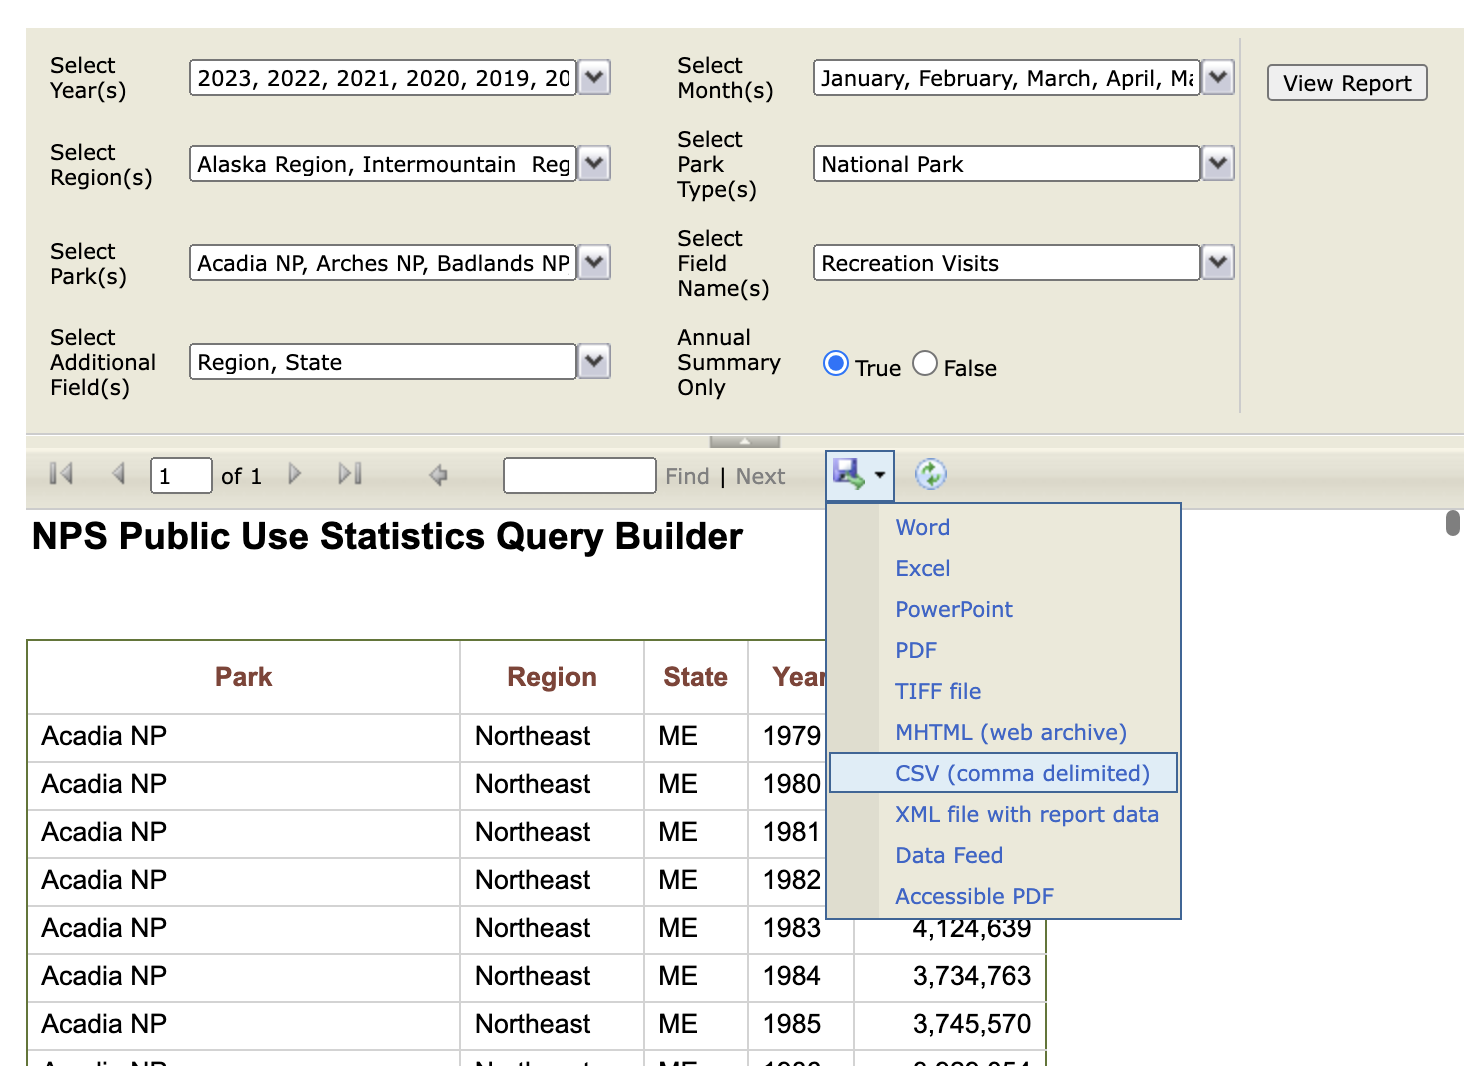
\includegraphics{query-builder-csv-screenshot.png}

\subsection{Why was the data collected? How is the data
used?}\label{why-was-the-data-collected-how-is-the-data-used}

As we've already discussed, one of the reasons that the NPS collects
visit data is because the government basically requires it. But there
are a lot of other reasons that the NPS collects this information.

As the NPS writes on their website, they use visit data to determine
which facilities might need more or less attention, which parks might
need more or less staff members and programs, and which hiking trails or
bathrooms might need more or less maintenance. This information also
helps the communities and businesses surrounding the parks understand
how they can best share and support resources in a given area
---~services like emergency vehicles, sanitation, and water. If there
are millions more people going on hikes in a particular area, and thus,
inevitably, many more people requiring ambulance trips or rescue
helicopters, that would be a very important thing for a community to
know. It would be dangerous if visitors to National Parks suddenly and
unexpectedly called all the emergency vehicles in town.

This visitation data also helps the NPS estimate the beneficial impact,
economic and otherwise, that the parks have on nearby communities and
the nation at large. These estimations are important because they help
the parks advocate for more funding, support, attention, and
collaboration.

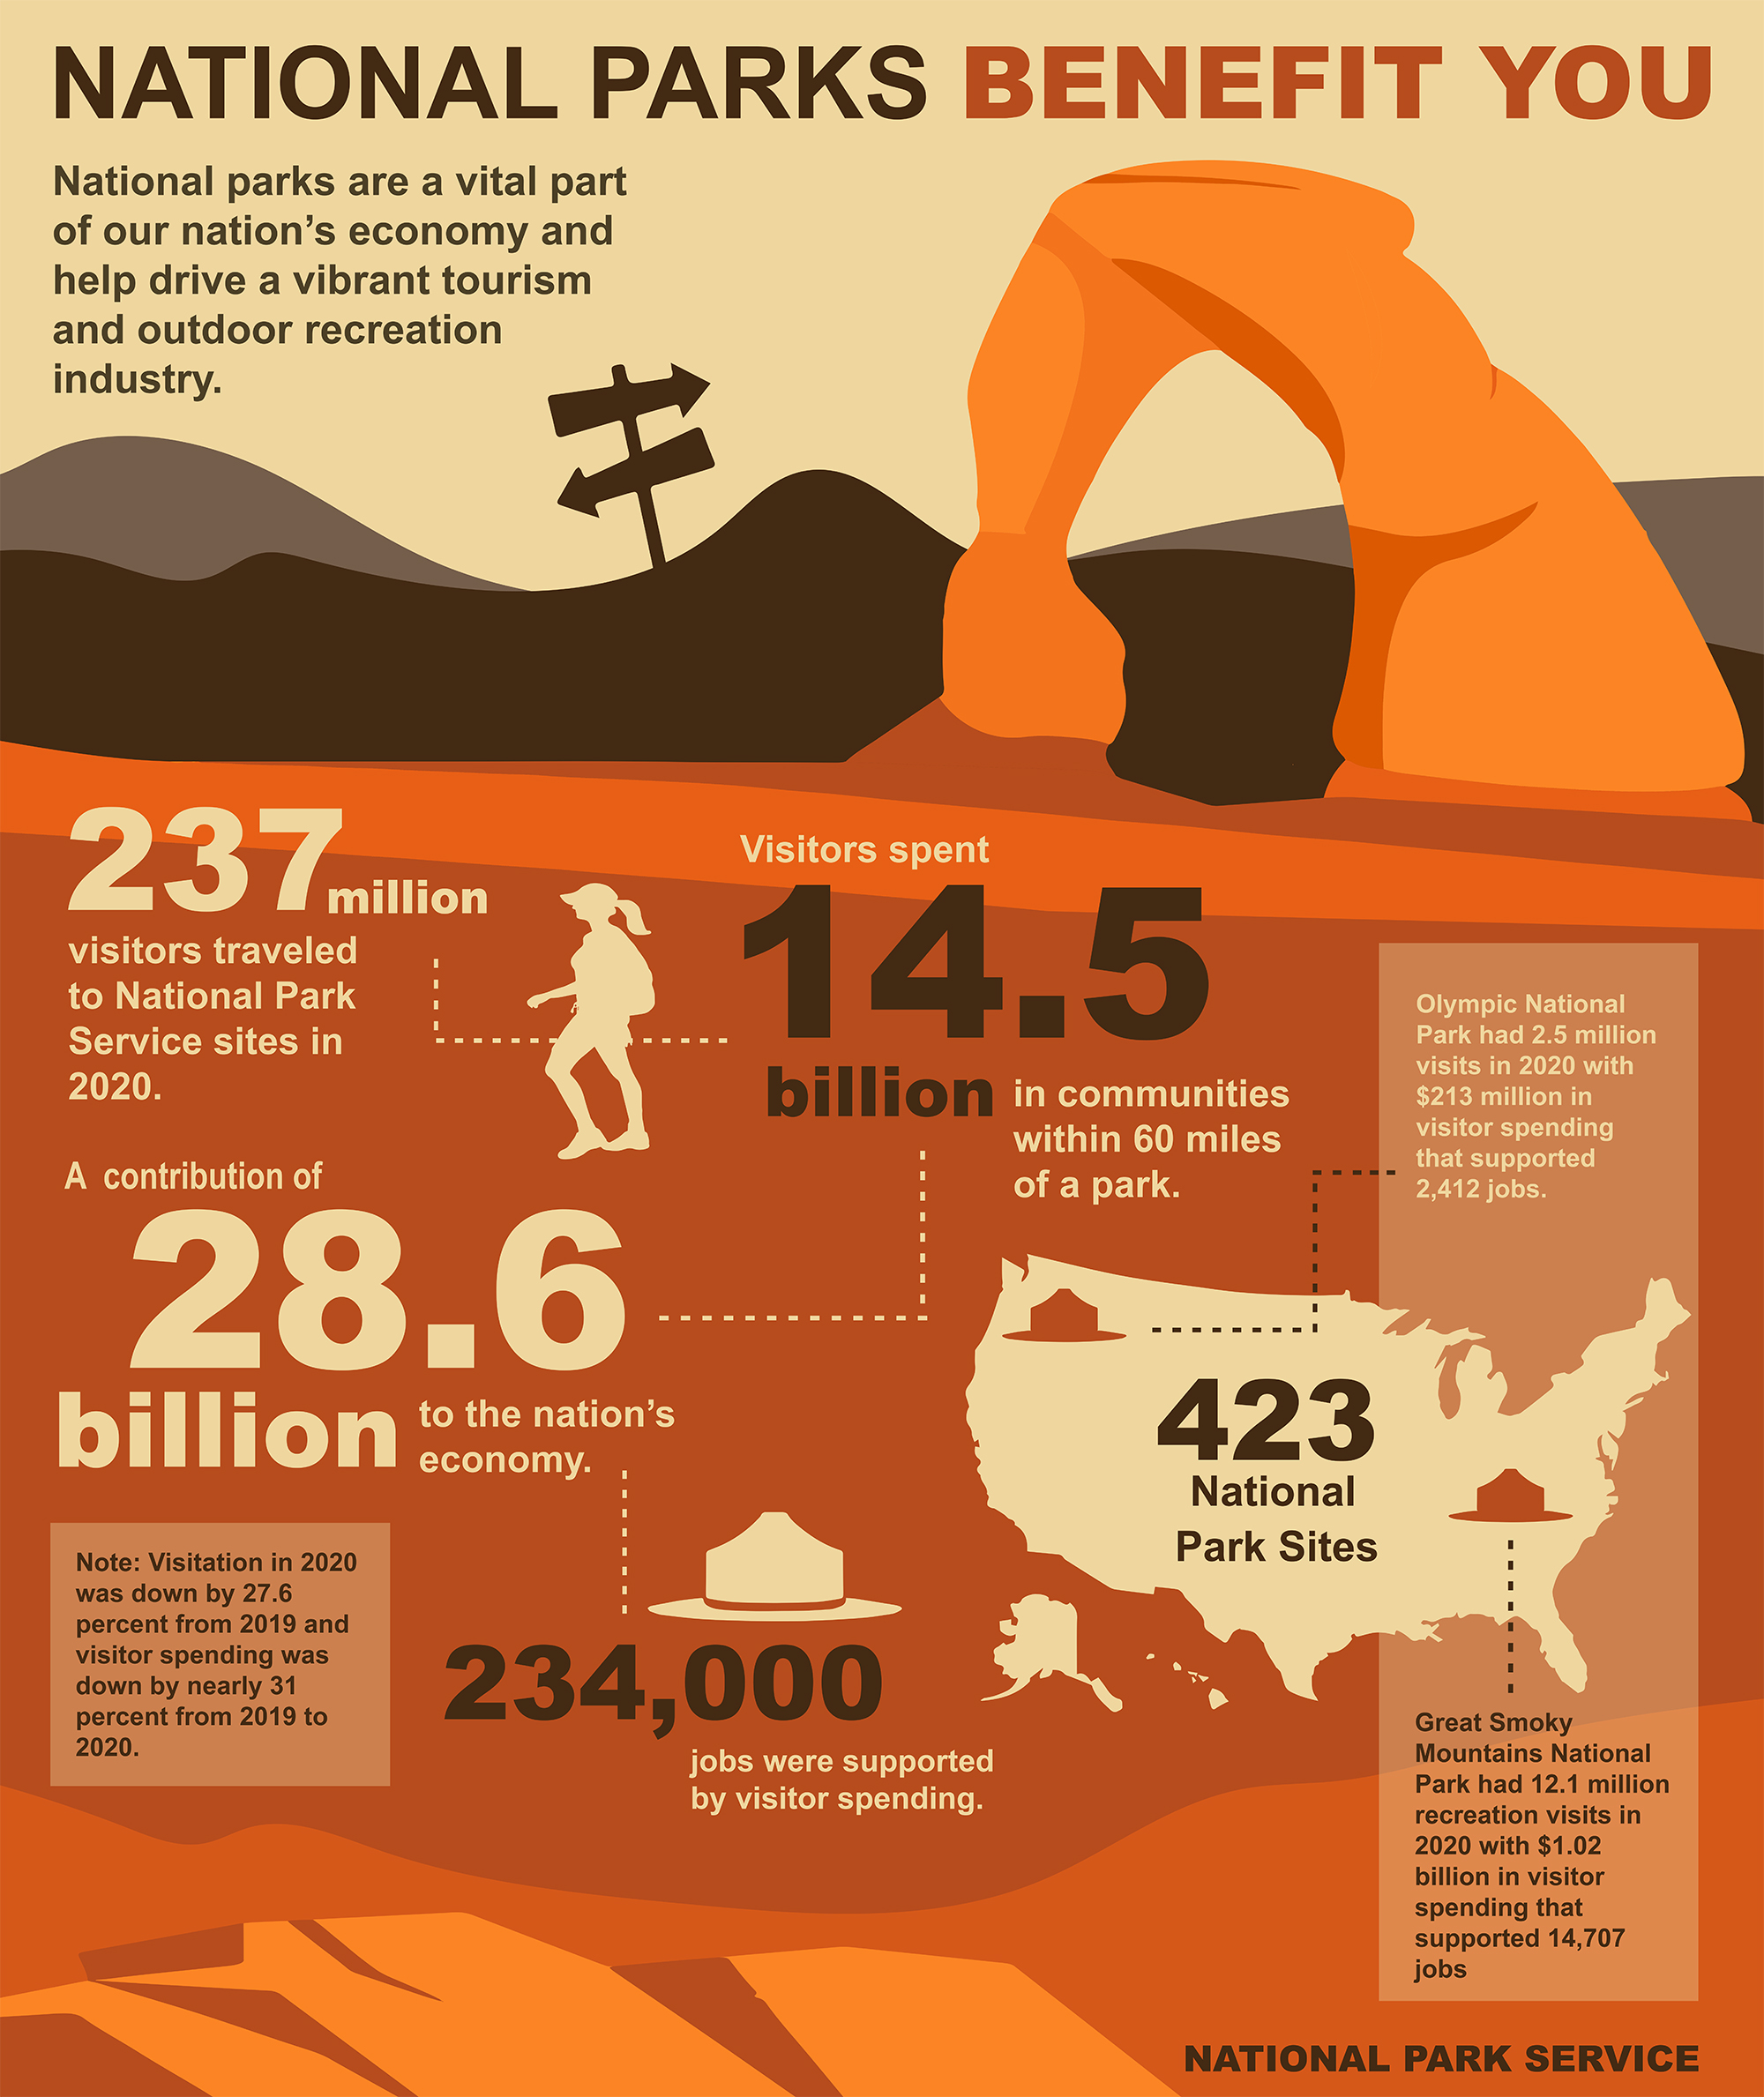
\includegraphics[width=3.125in,height=\textheight]{NP-economic-benefit-poster.jpg}

The data can also be used for a variety of other purposes\ldots. (such
as?)

\subsection{What's in the data? What ``counts'' as a
visit?}\label{whats-in-the-data-what-counts-as-a-visit}

If we open the dataset and look at the first few rows, we will find five
columns -- ``ParkName'', ``Region'', ``State'', ``Year'', and
``RecreationVisits'':

\begin{Shaded}
\begin{Highlighting}[]
\CommentTok{\# https://statsandr.com/blog/an{-}efficient{-}way{-}to{-}install{-}and{-}load{-}r{-}packages/}

\CommentTok{\# Load the dplyr package}
\FunctionTok{library}\NormalTok{(dplyr, }\AttributeTok{warn =} \ConstantTok{FALSE}\NormalTok{)}

\CommentTok{\# Load National Park Visitation data}
\NormalTok{np\_data }\OtherTok{\textless{}{-}} \FunctionTok{read.csv}\NormalTok{(}\StringTok{"https://raw.githubusercontent.com/melaniewalsh/Neat{-}Datasets/main/1979{-}2020{-}National{-}Park{-}Visits{-}By{-}State.csv"}\NormalTok{, }\AttributeTok{stringsAsFactors =} \ConstantTok{FALSE}\NormalTok{)}

\DocumentationTok{\#\# Look at the structure of the dataset}
\NormalTok{np\_data }\SpecialCharTok{\%\textgreater{}\%} \FunctionTok{slice\_sample}\NormalTok{(}\AttributeTok{n =} \DecValTok{10}\NormalTok{)}
\end{Highlighting}
\end{Shaded}

\begin{longtable}[]{@{}
  >{\raggedright\arraybackslash}p{(\columnwidth - 8\tabcolsep) * \real{0.3913}}
  >{\raggedright\arraybackslash}p{(\columnwidth - 8\tabcolsep) * \real{0.2029}}
  >{\raggedright\arraybackslash}p{(\columnwidth - 8\tabcolsep) * \real{0.0870}}
  >{\raggedleft\arraybackslash}p{(\columnwidth - 8\tabcolsep) * \real{0.0725}}
  >{\raggedleft\arraybackslash}p{(\columnwidth - 8\tabcolsep) * \real{0.2464}}@{}}
\toprule\noalign{}
\begin{minipage}[b]{\linewidth}\raggedright
ParkName
\end{minipage} & \begin{minipage}[b]{\linewidth}\raggedright
Region
\end{minipage} & \begin{minipage}[b]{\linewidth}\raggedright
State
\end{minipage} & \begin{minipage}[b]{\linewidth}\raggedleft
Year
\end{minipage} & \begin{minipage}[b]{\linewidth}\raggedleft
RecreationVisits
\end{minipage} \\
\midrule\noalign{}
\endhead
\bottomrule\noalign{}
\endlastfoot
Isle Royale NP & Midwest & MI & 1987 & 31760 \\
Great Sand Dunes NP \& PRES & Intermountain & CO & 2010 & 283284 \\
Bryce Canyon NP & Intermountain & UT & 2010 & 1285492 \\
Channel Islands NP & Pacific West & CA & 1993 & 184867 \\
Grand Canyon NP & Intermountain & AZ & 1994 & 4364316 \\
Death Valley NP & Pacific West & CA & 2006 & 744440 \\
Big Bend NP & Intermountain & TX & 2005 & 398583 \\
Guadalupe Mountains NP & Intermountain & TX & 2019 & 188833 \\
Dry Tortugas NP & Southeast & FL & 1981 & 10150 \\
Sequoia NP & Pacific West & CA & 1996 & 838060 \\
\end{longtable}

The first four are self-explanatory: but why is the fifth labelled
``RecreationVisits'' rather than ``Visits'', or ``Visitors''?

The answer is that what this dataset is tracking is more complicated and
nuanced than ``people who go to NPS properties''. People go to the
national parks for a lot of reasons. While many are there for
recreation, some travel \emph{through} the parks, either because a
highway runs through or because they live on ``inholdings'' (private
property that is surrounded by a national park on all sides). Because of
this,
\href{https://www.nps.gov/subjects/socialscience/nps-visitor-use-statistics-definitions.htm}{the
NPS defines} ``Recreation Visits'' as visits made by people who are
\emph{not}:

\begin{quote}
using park territory, roads, and facilities for their own convenience or
as a part of their occupation. \textgreater{} Reportable non-recreation
visits include:

\begin{itemize}
\tightlist
\item
  Persons going to and from inholdings across significant parts of park
  land;
\item
  Commuter and other traffic using NPS-administered roads or waterways
  through a park for their convenience;
\item
  Trades-people with business in the park;
\item
  Any civilian activity a part of or incidental to the pursuit of a
  gainful occupation (e.g., guides);
\item
  Government personnel (other than NPS employees) with business in the
  park;
\item
  Citizens using NPS buildings for civic or local government business,
  or attending public hearings;
\item
  Outside research activities (visits and overnights) if independent of
  NPS legislated interests (e.g.~meteorological research).
\end{itemize}
\end{quote}

What this means is that the counts leave out a lot of people. This is
worth thinking about when we evaluate what the numbers mean, and how the
NPS achieves them (which we'll discuss more below)

\subsection{Data and data collection}\label{data-and-data-collection}

So now we know what is being collected. But let's try to understand
\emph{how} it's being collected. We can do this, in part, by exploring
and visualising the data.

For example: let's visualise the visits to Crater Lakes National Park,
from 1979 to the present:

\begin{Shaded}
\begin{Highlighting}[]
\CommentTok{\# Load the "ggplot2" package (which we\textquotesingle{}ll be using a lot more)}
\FunctionTok{library}\NormalTok{(ggplot2)}

\CommentTok{\# Let\textquotesingle{}s also load "ggthemes", which let\textquotesingle{}s us use colorblind{-}compatible palettes. When we\textquotesingle{}ve only got one line, this will just be black.}
\FunctionTok{library}\NormalTok{(ggthemes)}

\CommentTok{\# And specify the colorblind palette}
\NormalTok{cb\_palette }\OtherTok{\textless{}{-}} \FunctionTok{colorblind\_pal}\NormalTok{()(}\DecValTok{8}\NormalTok{)}

\CommentTok{\# Turn off scientific notation}
\FunctionTok{options}\NormalTok{(}\AttributeTok{scipen =} \DecValTok{999}\NormalTok{)}

\CommentTok{\# Filter down to Crater Lake National Park}
\NormalTok{crater\_lake }\OtherTok{\textless{}{-}}\NormalTok{ np\_data }\SpecialCharTok{\%\textgreater{}\%} \FunctionTok{filter}\NormalTok{(ParkName }\SpecialCharTok{==} \StringTok{"Crater Lake NP"}\NormalTok{)}

\CommentTok{\# Visualize it}
\FunctionTok{ggplot}\NormalTok{(}\AttributeTok{data =}\NormalTok{ crater\_lake) }\SpecialCharTok{+} 
  \FunctionTok{geom\_line}\NormalTok{(}\FunctionTok{aes}\NormalTok{(}\AttributeTok{x =} 
\NormalTok{  Year, }\AttributeTok{y =}\NormalTok{ RecreationVisits), }
  \AttributeTok{color =}\NormalTok{ cb\_palette[}\DecValTok{1}\NormalTok{]) }\SpecialCharTok{+}
  \FunctionTok{labs}\NormalTok{(}\AttributeTok{title =} \StringTok{"Crater Lake National Park Visits (1979 {-} Present)"}\NormalTok{)}
\end{Highlighting}
\end{Shaded}

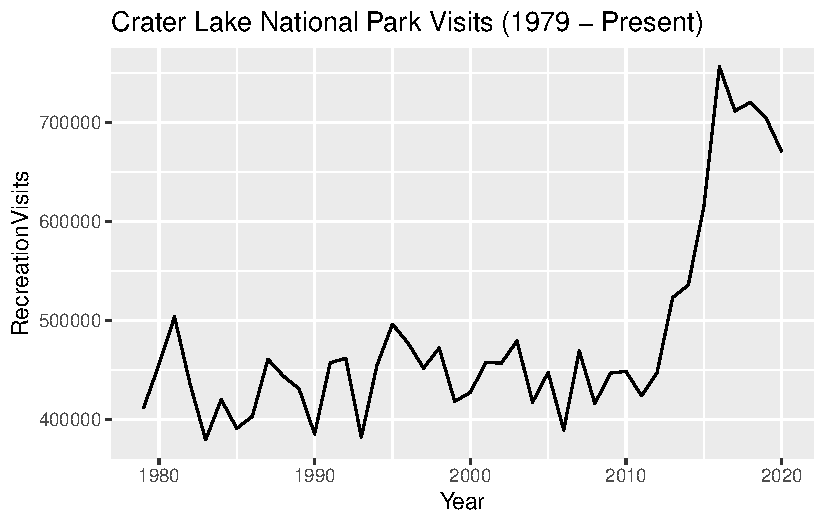
\includegraphics{index_files/figure-pdf/unnamed-chunk-3-1.pdf}

We see a lot of things in this data - not least of which is a tremendous
rise in visitors in the 2010s - but one interesting observation is the
sudden drop in visits in 2012. This isn't caused by fewer people
visiting: instead, it has more to do with how visitor numbers are
counted.

When it comes to counting visitors, the NPS uses a variety of
techniques. At some parks, such as Alcatraz, it is simple: the park is
only accessible via (ticketed) boat, and so NPS staff simply count the
number of tickets. But other parks may have multiple entrances, and
feature visitors arriving via car, bus, or on foot. It quickly becomes
impractical to have staff at every entrance, 24 hours a day, just in
case someone arrives.

Instead, the NPS uses a variety of techniques - some automated, some
manual. These include:

\begin{itemize}
\tightlist
\item
  Induction loop counters - magnetised coils of wire under the road that
  ``trip'' when a vehicle passes over them;
\item
  Traffic counters, which manually increment a counter when a vehicle
  passes through a gate;
\item
  Extracting data from ticketing machines.
\end{itemize}

\begin{figure}[H]

{\centering \includegraphics[width=3.125in,height=\textheight]{index_files/mediabag/Inductance_detectors.jpg}

}

\caption{An example of an induction loop installed under a road}

\end{figure}%

Alongside all of that, NPS rangers do, on many occasions, manually count
people who arrive - particularly when one of the usual mechanisms
doesn't count. And that's exactly what happened here;
\href{https://irma.nps.gov/Stats/SSRSReports/Park\%20Specific\%20Reports/Monthly\%20Visitation\%20Comments\%20By\%20Park?Park=CRLA}{according
to the NPS data logs}, the induction loop counter at one of the main
entrances simply broke in January, and wasn't repaired for (at a
minimum) several months. You can see a similar, but more severe, example
at Carlsbad Caverns National Park, where it appears visits entirely tail
off in 2020, as a result of
\href{https://irma.nps.gov/Stats/SSRSReports/Park\%20Specific\%20Reports/Monthly\%20Visitation\%20Comments\%20By\%20Park?Park=CRLA}{the
traffic counter being broken} for \emph{years}:

\begin{Shaded}
\begin{Highlighting}[]
\CommentTok{\# Filter down to Carlsbad Caverns National Park}
\NormalTok{carlsbad\_data }\OtherTok{\textless{}{-}}\NormalTok{ np\_data }\SpecialCharTok{\%\textgreater{}\%} \FunctionTok{filter}\NormalTok{(ParkName }\SpecialCharTok{==} \StringTok{"Carlsbad Caverns NP"}\NormalTok{)}

\CommentTok{\# Visualise it}
\FunctionTok{ggplot}\NormalTok{(}\AttributeTok{data =}\NormalTok{ carlsbad\_data) }\SpecialCharTok{+} 
  \FunctionTok{geom\_line}\NormalTok{(}\FunctionTok{aes}\NormalTok{(}\AttributeTok{x =}\NormalTok{ Year, }\AttributeTok{y =}\NormalTok{ RecreationVisits), }\AttributeTok{color =}\NormalTok{ cb\_palette[}\DecValTok{2}\NormalTok{]) }\SpecialCharTok{+} 
  \FunctionTok{labs}\NormalTok{(}\AttributeTok{title =} \StringTok{"Carlsbad Caverns National Park Visits (1979 {-} Present)"}\NormalTok{)}
\end{Highlighting}
\end{Shaded}

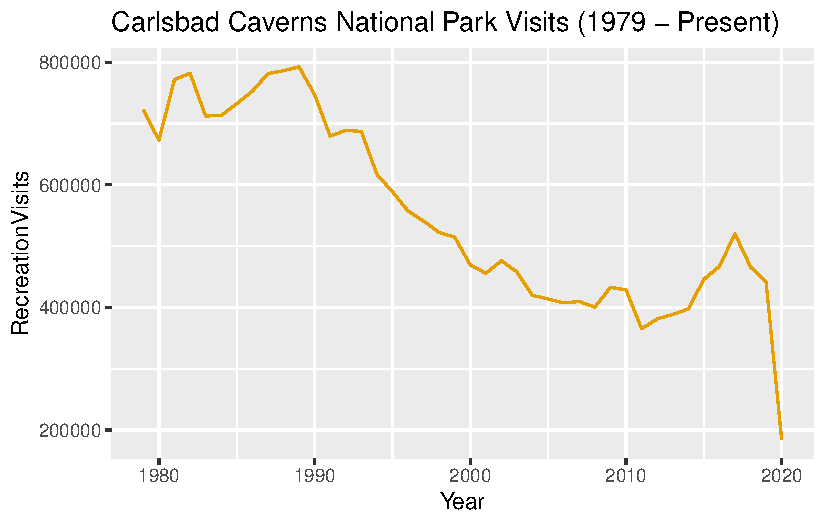
\includegraphics{index_files/figure-pdf/unnamed-chunk-4-1.pdf}

\subsection{Exercise: thinking about where (and how, and why) mechanisms
are likely to
break}\label{exercise-thinking-about-where-and-how-and-why-mechanisms-are-likely-to-break}

Now that we've talked about how data is collected (and the fragility of
some of those methods), it's a good time to think about how even the
same method, deployed at different places, might be differently
unreliable. For more, see \hyperref[exercise-1]{Exercise 1}.

\subsection{Data and reality}\label{data-and-reality}

Changes in data don't only stem from changes in data collection, but
also the underlying reality of what is being measured. Let's take a look
at the visitor data from Kobuk Valley National Park:

\begin{Shaded}
\begin{Highlighting}[]
\CommentTok{\# Filter down to Kobuk Valley National Park}
\NormalTok{kobuk\_data }\OtherTok{\textless{}{-}}\NormalTok{ np\_data }\SpecialCharTok{\%\textgreater{}\%} \FunctionTok{filter}\NormalTok{(ParkName }\SpecialCharTok{==} \StringTok{"Kobuk Valley NP"}\NormalTok{)}

\CommentTok{\# Visualise it}
\FunctionTok{ggplot}\NormalTok{(}\AttributeTok{data =}\NormalTok{ kobuk\_data) }\SpecialCharTok{+} 
  \FunctionTok{geom\_line}\NormalTok{(}\FunctionTok{aes}\NormalTok{(}\AttributeTok{x =}\NormalTok{ Year, }\AttributeTok{y =}\NormalTok{ RecreationVisits ), }\AttributeTok{color =}\NormalTok{ cb\_palette[}\DecValTok{3}\NormalTok{]) }\SpecialCharTok{+}
  \FunctionTok{labs}\NormalTok{(}\AttributeTok{title =} \StringTok{"Kobuk Valley National Park Visits (1979 {-} Present)"}\NormalTok{)}
\end{Highlighting}
\end{Shaded}

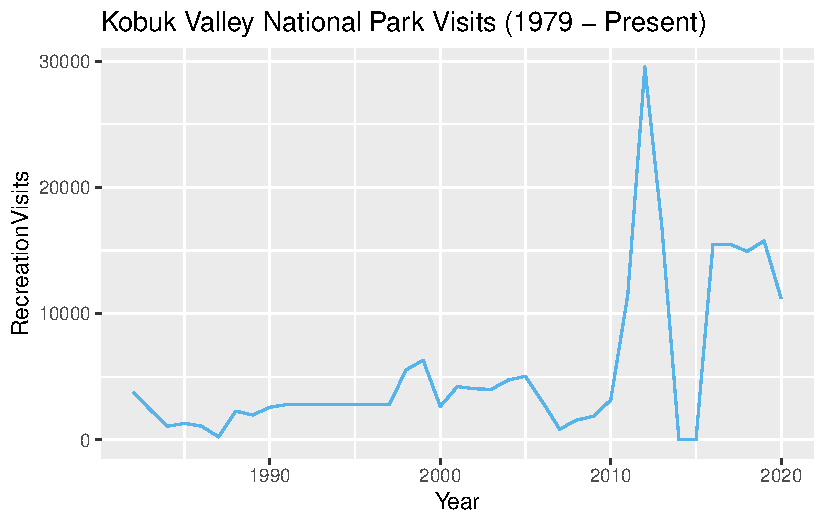
\includegraphics{index_files/figure-pdf/unnamed-chunk-5-1.pdf}

Most people's eyes will immediately be drawn to the drastic drop in
2014-15, and for good reason! But the cause is familiar: it's about data
collection. As the park report notes, ''
\href{https://irma.nps.gov/Stats/SSRSReports/Park\%20Specific\%20Reports/Monthly\%20Visitation\%20Comments\%20By\%20Park?Park=MORA}{The
park is developing a new counting system and has made the decision not
to report visitor counts until the new system is in place.}``.

But another question would be: why the drop-off in 2018-19? It's too
early for the cause to be COVID. Instead, the cause is administrative;
government shut-downs in that era led to a reduction of funding, and
correspondingly the closure of various attractions at the park. The
result: a lack of funding leads to a reduced visitor count - a visitor
count that is often used, remember, to \emph{argue for funding}. This
highlights one of the ways in which seemingly-descriptive data used to
make decisions can represent the state of those decisions, more than
some natural ``baseline''.

Another kind of issue of ``representing reality'' can be found if we
look at the visitor data for Mount Rainier:

\begin{Shaded}
\begin{Highlighting}[]
\CommentTok{\# Filter down to Mount Rainier National Park}
\NormalTok{rainier\_data }\OtherTok{\textless{}{-}}\NormalTok{ np\_data }\SpecialCharTok{\%\textgreater{}\%} \FunctionTok{filter}\NormalTok{(ParkName }\SpecialCharTok{==} \StringTok{"Mount Rainier NP"}\NormalTok{)}

\CommentTok{\# Visualise it}
\FunctionTok{ggplot}\NormalTok{(}\AttributeTok{data =}\NormalTok{ rainier\_data) }\SpecialCharTok{+} 
  \FunctionTok{geom\_line}\NormalTok{(}\FunctionTok{aes}\NormalTok{(}\AttributeTok{x =}\NormalTok{ Year, }\AttributeTok{y =}\NormalTok{ RecreationVisits ), }\AttributeTok{color =}\NormalTok{ cb\_palette[}\DecValTok{4}\NormalTok{]) }\SpecialCharTok{+}
  \FunctionTok{labs}\NormalTok{(}\AttributeTok{title =} \StringTok{"Mount Rainier National Park Visits (1979 {-} Present)"}\NormalTok{)}
\end{Highlighting}
\end{Shaded}

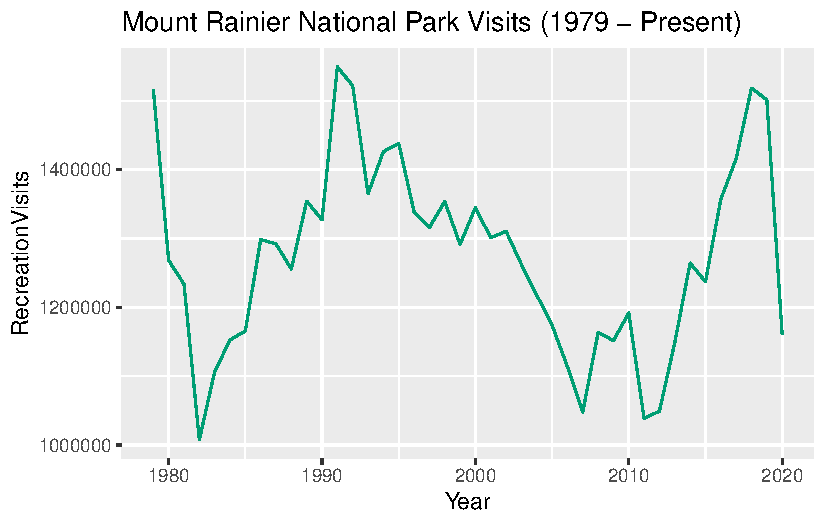
\includegraphics{index_files/figure-pdf/unnamed-chunk-6-1.pdf}

Once again, we see both a COVID-19 dropoff - but also a continued
dropoff beyond that.
\href{https://irma.nps.gov/Stats/SSRSReports/Park\%20Specific\%20Reports/Monthly\%20Visitation\%20Comments\%20By\%20Park?Park=MORA}{Looking
at the visitation comments} explains why; flooding, fires and a blizzard
drastically impeded the ability of people to get to the park, and the
possibility of areas of the park opening at all.

\subsection{Compensating for data}\label{compensating-for-data}

As all of this should suggest, NPS data is always somewhat approximate.
Reductions in funding, damage to counting equipment, natural events, or
simply the inevitably-fallible nature of \emph{any} data collection
means that data requires a certain amount of prediction, guesswork and
massaging to look complete.

Sometimes this leads to odd-looking decisions. For example: at
Assateague Island National Seashore, there are two entrances (one in
Maryland, and one in Virginia). At both entrances, they use a traffic
counter to count vehicles. At both entrances, they get from vehicles to
visitors by multiplying the number of vehicles by an estimate of how
many people each vehicle contains. But at the Maryland entrance, that's
2.9. At the Virginia entrance, it's 3.2.

\subsection{Exercise: compensating for data
outages}\label{exercise-compensating-for-data-outages}

\emph{Reader note: this exercise will direct students, on a group (or
individual) basis, to the NPS index of how different parks calculate
different multipliers and metrics, and ask them to log or note unusual
or unexplained differences in how this is done.}

\subsection{Data decisions}\label{data-decisions}

As well as multiplying up, there's also counting down: some parks
register ``zero'' as the number of visitors they attracted in a year:

\subsection{Look at the structure of the
dataset}\label{look-at-the-structure-of-the-dataset}

\begin{Shaded}
\begin{Highlighting}[]
\CommentTok{\# Filter down to just zeros}
\NormalTok{zero\_data }\OtherTok{\textless{}{-}}\NormalTok{ np\_data }\SpecialCharTok{\%\textgreater{}\%} \FunctionTok{filter}\NormalTok{(RecreationVisits }\SpecialCharTok{==} \DecValTok{0}\NormalTok{)}

\CommentTok{\# Show some of them}
\FunctionTok{slice\_sample}\NormalTok{(}\AttributeTok{.data =}\NormalTok{ zero\_data, }\AttributeTok{n =} \DecValTok{10}\NormalTok{)}
\end{Highlighting}
\end{Shaded}

\begin{longtable}[]{@{}
  >{\raggedright\arraybackslash}p{(\columnwidth - 8\tabcolsep) * \real{0.4384}}
  >{\raggedright\arraybackslash}p{(\columnwidth - 8\tabcolsep) * \real{0.1781}}
  >{\raggedright\arraybackslash}p{(\columnwidth - 8\tabcolsep) * \real{0.0822}}
  >{\raggedleft\arraybackslash}p{(\columnwidth - 8\tabcolsep) * \real{0.0685}}
  >{\raggedleft\arraybackslash}p{(\columnwidth - 8\tabcolsep) * \real{0.2329}}@{}}
\toprule\noalign{}
\begin{minipage}[b]{\linewidth}\raggedright
ParkName
\end{minipage} & \begin{minipage}[b]{\linewidth}\raggedright
Region
\end{minipage} & \begin{minipage}[b]{\linewidth}\raggedright
State
\end{minipage} & \begin{minipage}[b]{\linewidth}\raggedleft
Year
\end{minipage} & \begin{minipage}[b]{\linewidth}\raggedleft
RecreationVisits
\end{minipage} \\
\midrule\noalign{}
\endhead
\bottomrule\noalign{}
\endlastfoot
Kobuk Valley NP & Alaska & AK & 2014 & 0 \\
National Park of American Samoa & Pacific West & AS & 2003 & 0 \\
Kobuk Valley NP & Alaska & AK & 2015 & 0 \\
Katmai NP \& PRES & Alaska & AK & 1995 & 0 \\
\end{longtable}

Looking at the parks and regions, we can maybe infer why; they are all
in extremely rural or underresourced areas, and probably see few
visitors to begin with. If we look at the visitors over time for one
park that has ``zero counts'', Kobuk Valley National park, we see it's
hardly overrun with people even when the count \emph{isn't} zero:

\begin{Shaded}
\begin{Highlighting}[]
\CommentTok{\# Filter down to Mount Rainier National Park}
\NormalTok{kobuk\_data }\OtherTok{\textless{}{-}}\NormalTok{ np\_data }\SpecialCharTok{\%\textgreater{}\%} \FunctionTok{filter}\NormalTok{(ParkName }\SpecialCharTok{==} \StringTok{"Kobuk Valley NP"}\NormalTok{)}

\CommentTok{\# Visualise it}
\FunctionTok{ggplot}\NormalTok{(}\AttributeTok{data =}\NormalTok{ kobuk\_data) }\SpecialCharTok{+} 
  \FunctionTok{geom\_line}\NormalTok{(}\FunctionTok{aes}\NormalTok{(}\AttributeTok{x =}\NormalTok{ Year, }\AttributeTok{y =}\NormalTok{ RecreationVisits ), }\AttributeTok{color =}\NormalTok{ cb\_palette[}\DecValTok{6}\NormalTok{]) }\SpecialCharTok{+}
  \FunctionTok{labs}\NormalTok{(}\AttributeTok{title =} \StringTok{"Kobuk Valley National Park Visits (1979 {-} Present)"}\NormalTok{)}
\end{Highlighting}
\end{Shaded}

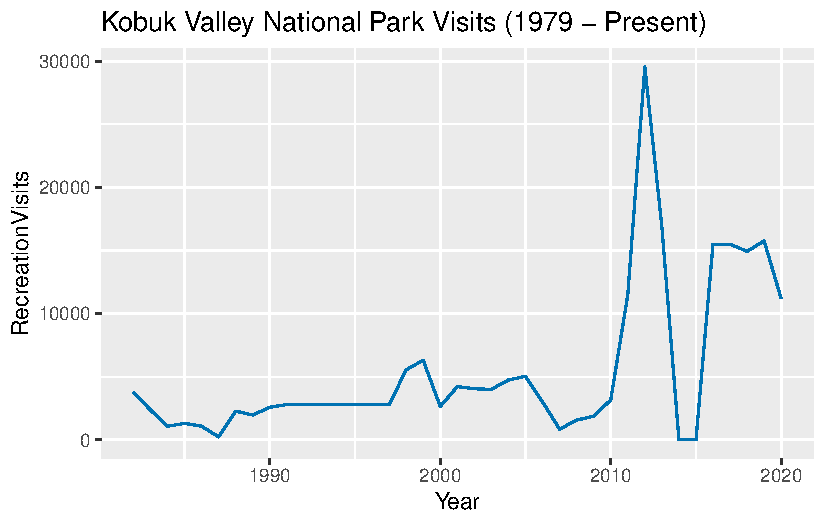
\includegraphics{index_files/figure-pdf/unnamed-chunk-8-1.pdf}

If we look at the visitation comments again,
\href{https://irma.nps.gov/Stats/SSRSReports/Park\%20Specific\%20Reports/Monthly\%20Visitation\%20Comments\%20By\%20Park}{what
we see} is that ``The park is developing a new counting system and has
made the decision not to report visitor counts until the new system is
in place.'' Which is entirely reasonable, in isolation: but we've also
seen a \emph{lot} of parks in more highly-frequented areas that have new
systems developed and choose to (for example) average previous years,
rather than simply declare that nobody visited. What are the politics of
the choices in these scenarios?

\subsection{Exercise: data decisions}\label{exercise-data-decisions}

\emph{Reader note: in this exercise, users will try to use public data -
twitter posts, flickr photos, etc, etc - to try and find situations
where people are identifying themselves as being at a park that,
officially, has 0 people present at that time Have them go through
public data and try to find proof the counts of 0 are ``wrong''}

\section{Explore the Data}

\begin{Shaded}
\begin{Highlighting}[]
\NormalTok{//| echo: false}
\NormalTok{viewof search = Inputs.search(data, \{}
\NormalTok{  placeholder: "Search"}
\NormalTok{\})}
\end{Highlighting}
\end{Shaded}

\begin{Shaded}
\begin{Highlighting}[]
\NormalTok{//| echo: false}
\NormalTok{//| output: false}
\NormalTok{data = d3.csv("https://raw.githubusercontent.com/melaniewalsh/Neat{-}Datasets/main/1979{-}2022{-}National{-}Park{-}Visits{-}By{-}State.csv", d3.autoType)}
\end{Highlighting}
\end{Shaded}

\begin{Shaded}
\begin{Highlighting}[]
\NormalTok{//| echo: false}
\NormalTok{//| output: false}


\NormalTok{filtered = data.filter(function(penguin) \{}
\NormalTok{  return bill\_length\_min \textless{} penguin.bill\_length\_mm \&\&}
\NormalTok{         islands.includes(penguin.island);}
\NormalTok{\})}
\end{Highlighting}
\end{Shaded}

\begin{Shaded}
\begin{Highlighting}[]
\NormalTok{//| echo: false}
\NormalTok{color = d3}
\NormalTok{  .scaleLinear()}
\NormalTok{  .domain([5000000, 1000000, 100000])}
\NormalTok{  .range(["\#cafcc2", "\#fce7c2", "\#eb9494"])}
\end{Highlighting}
\end{Shaded}

\begin{Shaded}
\begin{Highlighting}[]
\NormalTok{//| echo: false}

\NormalTok{/*Inputs.table(search, data)*/}

\NormalTok{Inputs.table(search, \{}
\NormalTok{  layout: "fixed",}
\NormalTok{  rows: 50,}
\NormalTok{  sort: "Year",}
\NormalTok{  reverse: true,}
\NormalTok{  format: \{}
\NormalTok{    /*RecreationVisits: x =\textgreater{} d3.format(\textquotesingle{}.2s\textquotesingle{})(x),*/}
\NormalTok{    Year: x =\textgreater{} d3.timeFormat(x),}
\NormalTok{    RecreationVisits: x =\textgreater{} html\textasciigrave{}\textless{}div style=\textquotesingle{}background:$\{color(x)\}\textquotesingle{}\textgreater{}$\{d3.format(\textquotesingle{}.2s\textquotesingle{})(x)\}\textless{}/div\textgreater{}\textasciigrave{}}
\NormalTok{  \}}
\NormalTok{\})}
\end{Highlighting}
\end{Shaded}

\section{Exercises}

\section{R}

\phantomsection\label{exercise-posts}

\section{Python}

\section{Discussion \& Activities}

\subsection{Activity 1}\label{exercise-1}

Devices breaking is inevitable - but as the different scales of the
Carlsbad and Crater Lake outages indicate, they get \emph{fixed} at
different rates, in different locations. There are a lot of reasons for
this, but some of the big ones might be geography and resources. The
more remote a park, the harder it is to get a repair team to it---and
the less-resourced a park, the lower the likelihood they have on-site
repair teams, or are prioritised by the repair teams that can be
dispatched.

Thinking about this, look at the locations of the following parks.
Suppose that each one has an outage in their induction loop: which ones
would you expect to be fixed first, and why? Research the parks, and
rank them on a scale of 1 to 5 (1 being highest, and 5 being lowest) of
which would be fixed quickest.

\begin{longtable}[]{@{}lll@{}}
\toprule\noalign{}
Park & Priority (1-5) & Reason \\
\midrule\noalign{}
\endhead
\bottomrule\noalign{}
\endlastfoot
Acadia NP & & \\
Lassen Volcanic NP & & \\
Saguaro NP & & \\
Yosemite NP & & \\
Mammoth Cave NP & & \\
\end{longtable}



\end{document}
